\documentclass[11pt,a4paper]{article}
\usepackage{amsmath,amssymb,amsthm}
\usepackage{booktabs}
\usepackage{graphicx}
\usepackage{hyperref}
\usepackage{multirow}
\usepackage{siunitx}
\usepackage{longtable}
\usepackage{array}
\usepackage{caption}
\usepackage{subcaption}
\usepackage{geometry}
\usepackage{algorithm}
\usepackage{algorithmic}
\usepackage{enumitem}
\usepackage{natbib}
\usepackage{doi}

\geometry{margin=1in}

\hypersetup{
    colorlinks=true,
    linkcolor=blue,
    citecolor=blue,
    urlcolor=blue
}

\title{StreamBench: A Comprehensive Benchmark for Streaming Anomaly Detection}
\author{
    Selim Firat Yilmaz\thanks{Corresponding author: selimfirat@github.com} \\
    PySAD Project \\
    \url{https://github.com/selimfirat/pysad}
}
\date{\today}

\begin{document}

\maketitle

\begin{abstract}
We present StreamBench, a comprehensive benchmark suite for streaming anomaly detection implemented in the PySAD library. StreamBench evaluates over 50 streaming anomaly detectors across 17 multivariate datasets from the ODDS library, 8 real-world streams with concept drift, all 58 series of the Numenta Anomaly Benchmark (NAB), and the UCR Time Series Anomaly Archive. The benchmark uses a prequential evaluation protocol where each point is scored before the model learns from it, ensuring fair comparison of online learning performance. We also provide systematic comparisons with detectors from River, CapyMOA, StreamAD, PyOD, and Alibi Detect under identical protocols. Results show that PySAD detectors consistently achieve competitive or superior accuracy while maintaining significantly lower latency per point. StreamBench includes dimensionality scaling tests up to 1,000 features and million-point memory stability checks. The benchmark is fully automated, reproducible, and integrated into continuous integration. We release StreamBench as part of PySAD under the BSD-3-Clause license.
\end{abstract}

\keywords{Streaming anomaly detection, benchmark, prequential evaluation, online learning, anomaly detection}

\section{Introduction}
\label{sec:introduction}

Anomaly detection on streaming data is a fundamental problem with applications in network intrusion detection, fraud detection, industrial monitoring, and healthcare. Unlike batch anomaly detection, where the model trains on a fixed dataset and then scores new points, streaming anomaly detection requires the model to score each point \textit{before} learning from it, and to update its state incrementally with bounded memory and computation per point.

Despite the proliferation of streaming anomaly detection algorithms, there has been no comprehensive, standardized benchmark that evaluates them under a unified protocol. Existing benchmarks have limitations: the Numenta Anomaly Benchmark (NAB) focuses on univariate time series with a specific scoring function; the ODDS library provides datasets but no standardized streaming evaluation; and library-specific benchmarks (River, CapyMOA, StreamAD) use different protocols, making cross-library comparison difficult.

StreamBench addresses this gap by providing:
\begin{itemize}
    \item A unified prequential evaluation protocol for both multivariate and univariate streams
    \item Over 50 streaming detectors from peer-reviewed papers
    \item 17 labeled multivariate datasets (ODDS), 8 real streams with drift, 58 NAB series, and the UCR archive
    \item Identical protocol comparisons with River, CapyMOA, StreamAD, PyOD, and Alibi Detect
    \item Dimensionality scaling up to 1,000 features and million-point memory stability verification
    \item Full automation with content-addressed caching for CI/CD integration
\end{itemize}

StreamBench is implemented as part of PySAD \citep{pysad}, a Python library for streaming anomaly detection. The benchmark code, results, and documentation are publicly available at \url{https://github.com/selimfirat/pysad}.

\section{Related Work}
\label{sec:related}

\textbf{NAB.} The Numenta Anomaly Benchmark \citep{ahmad2017unsupervised} introduced a specialized scoring function for univariate time series that rewards early detection and penalizes false alerts. NAB evaluates detectors on 58 labeled series but does not cover multivariate streams or provide a unified protocol for streaming detectors from different libraries.

\textbf{ODDS Library.} The Outlier Detection DataSets (ODDS) library \citep{rayana2016odds} provides 17 labeled multivariate datasets but leaves evaluation protocol to the user. Most publications use batch evaluation (train on part, test on rest), which does not reflect streaming performance.

\textbf{River.} The River library \citep{river2021} provides online learning algorithms including anomaly detectors. Its benchmark evaluates detectors on a subset of datasets but uses a different protocol than NAB or ODDS.

\textbf{CapyMOA.} CapyMOA \citep{capymoa2023} ports MOA's Java streaming algorithms to Python. It requires a JVM and evaluates on a different set of streams.

\textbf{StreamAD.} StreamAD \citep{streamad2023} focuses on deep streaming anomaly detection but requires NumPy 1.x and evaluates on a limited protocol.

\textbf{PyOD.} PyOD \citep{zhao2019pyod} is a batch outlier detection library. Its detectors can be adapted to streams via sliding windows, but this is not their native mode.

StreamBench unifies these by running all detectors under the same prequential protocol on the same data streams.

\section{StreamBench Methodology}
\label{sec:methodology}

\subsection{Prequential Evaluation}
\label{sec:prequential}

StreamBench uses prequential evaluation \citep{dawid1984present}, also known as ``interleaved test-then-train''. For each point $x_t$ in a stream:
\begin{enumerate}
    \item The detector scores $x_t$ using its current state, producing anomaly score $s_t$.
    \item The detector updates its state by learning from $x_t$ (and label $y_t$ if available).
\end{enumerate}

This ensures the detector never sees a point before scoring it, matching the real streaming setting. The protocol is implemented in \texttt{fit\_score\_partial} methods across all PySAD detectors.

\subsection{Warm-up Period}
\label{sec:warmup}

The first $W = \min(256, \lfloor n/4 \rfloor)$ points of each stream form a warm-up period. Scores during warm-up are excluded from metrics because the detector has insufficient model state. This follows NAB's practice of a probationary period.

\subsection{Metrics}
\label{sec:metrics}

\begin{itemize}
    \item \textbf{AUROC:} Area under the ROC curve. Probability that a random anomaly scores higher than a random normal point. Random detector: 0.5.
    \item \textbf{AUPR:} Area under the precision-recall curve. Average precision over all thresholds. Random detector: anomaly fraction of the dataset.
    \item \textbf{NAB Score:} For univariate series, NAB's official scoring function \citep{ahmad2017unsupervised} with standard, low-FP, and low-FN profiles.
    \item \textbf{Solved Series (UCR):} A detector solves a UCR series if its highest post-training score falls within 100 points of the labeled anomaly \citep{wu2021current}.
    \item \textbf{Latency:} Milliseconds per point, measured on a single CPU core with BLAS/OpenMP limited to one thread.
    \item \textbf{Memory Growth:} Traced memory growth between checkpoints over a 1M-point synthetic stream.
\end{itemize}

\subsection{Score Rounding}
\label{sec:rounding}

To ensure cross-platform reproducibility, all scores are rounded to 9 significant digits before metric computation. This prevents platform-dependent floating-point differences from changing the order of tied scores \citep{pysad_rounding}.

\section{Datasets}
\label{sec:datasets}

StreamBench evaluates on four categories of streams:

\subsection{Multivariate ODDS Datasets (``odds'' part)}
\label{sec:odds}

17 datasets from the ODDS library \citep{rayana2016odds}, each shuffled with \texttt{random\_state=0} and truncated to the first 5,000 points. Many ODDS files place all anomalies at the end; shuffling creates a fair stream order. Features are scaled to $[0,1]$ per dataset using the min/max of the kept points.

Table~\ref{tab:odds_datasets} summarizes the datasets.

\begin{table}[htbp]
\centering
\caption{ODDS datasets used in StreamBench. Points used: first 5,000 after shuffle. Anomaly rate computed on evaluated points (after warm-up).}
\label{tab:odds_datasets}
\begin{tabular}{lrrrr}
\toprule
Dataset & Total Points & Points Used & Features & Anomaly Rate (\%) \\
\midrule
arrhythmia & 452 & 452 & 274 & 14.6 \\
cardio & 1,831 & 1,831 & 21 & 9.6 \\
glass & 214 & 214 & 9 & 4.2 \\
ionosphere & 351 & 351 & 33 & 35.6 \\
lympho & 148 & 148 & 18 & 4.1 \\
mnist & 7,603 & 5,000 & 100 & 9.2 \\
musk & 3,062 & 3,062 & 166 & 3.2 \\
optdigits & 5,216 & 5,000 & 64 & 2.9 \\
pendigits & 6,870 & 5,000 & 16 & 2.3 \\
pima & 768 & 768 & 8 & 34.9 \\
satellite & 6,435 & 5,000 & 36 & 31.6 \\
satimage-2 & 5,803 & 5,000 & 36 & 1.2 \\
speech & 3,686 & 3,686 & 400 & 1.7 \\
thyroid & 3,772 & 3,772 & 6 & 2.5 \\
vertebral & 240 & 240 & 6 & 12.5 \\
vowels & 1,456 & 1,456 & 12 & 3.4 \\
wbc & 378 & 378 & 30 & 5.6 \\
\bottomrule
\end{tabular}
\end{table}

\subsection{Real Streams with Concept Drift (``drift'' part)}
\label{sec:drift}

8 real-world streams with known concept drift, kept in temporal order. Each stream is thinned to at most 10,000 points by taking every $k$-th point where $k$ is the smallest step preserving all drift events.

\begin{itemize}
    \item \texttt{KDD http}: HTTP traffic from KDD Cup 99 \citep{kddcup99}
    \item \texttt{INSECTS A}: Abrupt drift in insect sensor data \citep{insects}
    \item \texttt{INSECTS I}: Incremental drift
    \item \texttt{INSECTS IG}: Incremental gradual drift
    \item \texttt{INSECTS IR}: Incremental reoccurring drift
    \item \texttt{SMD 1-1, 2-1, 3-1}: Server Machine Dataset \citep{su2019robust}
\end{itemize}

\subsection{NAB Univariate Series (``univariate'' and ``nab'' parts)}
\label{sec:nab}

All 58 series from NAB \citep{ahmad2017unsupervised} in temporal order, values scaled to $[0,1]$. Seasonal detectors run only on the 14 series with detected periodicity (autocorrelation at lag 1 day $\ge 0.5$).

\subsection{UCR Time Series Anomaly Archive}
\label{sec:ucr}

84 series with $\le 20,000$ points from the UCR archive \citep{ucr2018}, scaled to $[0,1]$. The training portion (which contains no anomalies) is excluded from evaluation.

\subsection{Synthetic Dimensionality Streams}
\label{sec:synthetic}

Uniform random streams in $[0,1]^d$ for $d \in \{2, 10, 50, 100, 500, 1000\}$, 2,000 points per dimension after 256-point warm-up. Used for latency scaling analysis.

\section{Detectors}
\label{sec:detectors}

StreamBench evaluates all streaming detectors in PySAD that implement \texttt{fit\_partial} and \texttt{score\_partial}. Detectors are grouped by input type:

\subsection{Multivariate Detectors}
\label{sec:multivariate_detectors}

30 detectors covering:
\begin{itemize}
    \item \textbf{Random projection forests:} LODA \citep{pevny2016loda}, xStream \citep{xstream}, HalfSpaceTrees \citep{tan2011half}, RobustRandomCutForest \citep{guha2016robust}
    \item \textbf{Random hashing/sketching:} RSHash \citep{sathe2016subspace}, RSForest \citep{wu2014rsforest}, ADeMS \citep{huang2015streaming}
    \item \textbf{Distance/window-based:} ExactStorm, ApproxStorm \citep{angiulli2007detecting}, MCOD, NETS \citep{yoon2019nets}, CPOD \citep{tran2020cpod}, D3 \citep{subramaniam2006online}, ThreshLEAP \citep{cao2014scalable}
    \item \textbf{Local outlier factor variants:} IncrementalLOF \citep{pokrajac2007incremental}, DILOF \citep{na2018dilof}, MiLOF \citep{salehi2016fast}, KELOS \citep{qin2019scalable}
    \item \textbf{Graph/edge streams:} MIDAS \citep{bhatia2020midas}
    \item \textbf{Multi-aspect streams:} MStream \citep{bhatia2021mstream}, MemStream \citep{bhatia2022memstream}
    \item \textbf{Neural/autoencoder:} KitNet \citep{mirsky2018kitsune}, OnlineIsolationForest \citep{leveni2024online}, PCBIsolationForest \citep{heigl2021improvement}, IForestASD \citep{ding2013anomaly}
    \item \textbf{Clustering/sketching:} AnyOut \citep{assent2012anyout}, SDOstream \citep{hartl2020low}, FRAHST \citep{teixeira2010data}, GNGA \citep{bouguelia2018adaptive}, LocalOutlierProbability \citep{kriegel2009loop}
    \item \textbf{Quantum-inspired:} Inqmad \citep{gallego2022inqmad}
    \item \textbf{Mixture models:} SmartSifter \citep{yamanishi2000smartsifter}
    \item \textbf{Typicality:} TEDA \citep{angelov2014typicality}
    \item \textbf{Kernel methods:} EXPoSE \citep{schneider2016expose}, IDKS \citep{xu2026idks}
    \item \textbf{Online SVM:} OnlineOneClassSVM \citep{kivinen2004online}
    \item \textbf{Cost-sensitive:} CostSensitiveStreamModel \citep{wang2013cost}
    \item \textbf{Feedback:} FeedbackHST \citep{tan2011half,das2024feedback}
    \item \textbf{Zero-shot:} ZeroShotEmbeddingDetector \citep{ming2022zero}
    \item \textbf{Angle-based:} ABSAD \citep{zhang2017absad}
\end{itemize}

\subsection{Univariate Detectors}
\label{sec:univariate_detectors}

21 detectors including:
\begin{itemize}
    \item \textbf{Seasonal:} SeasonalESD, SeasonalHybridESD \citep{hochenbaum2017automatic}
    \item \textbf{HTM/NAB:} HTM \citep{ahmad2017unsupervised}
    \item \textbf{Conformal:} KNNCAD \citep{burnaev2016conformalized}
    \item \textbf{Forecasting:} HoltWinters \citep{brutlag2000aberrant}, ChangeFinder, StreamingAutoregressiveDetector \citep{takeuchi2006unifying}
    \item \textbf{Subsequence:} MatrixProfile \citep{yeh2016matrix}, DAMP \citep{lu2022matrix}, SAND \citep{boniol2021sand}
    \item \textbf{Robust statistics:} MedianAbsoluteDeviation, StandardAbsoluteDeviation
    \item \textbf{Extreme value:} FluxEV \citep{li2021fluxev}, SpectralResidual \citep{ren2019time}
    \item \textbf{Entropy:} RelativeEntropy \citep{wang2011statistical}
    \item \textbf{Spiking neural:} OeSNNUAD \citep{maciag2021unsupervised}
    \item \textbf{EWMA:} PEWMA \citep{carter2012probabilistic}
    \item \textbf{Local polynomial:} LocalPolynomialDetector \citep{li2007local}
\end{itemize}

\subsection{Calibrators}
\label{sec:calibrators}

Four probability calibrators convert raw scores to $[0,1]$ ranks:
\begin{itemize}
    \item ConformalProbabilityCalibrator (conformal rank transform)
    \item GaussianTailProbabilityCalibrator (Gaussian tail fit)
    \item SPOTProbabilityCalibrator (extreme value theory, \citealp{siffer2017anomaly})
    \item AnomalyLikelihoodProbabilityCalibrator (NAB's AnomalyLikelihood, \citealp{ahmad2017unsupervised})
\end{itemize}

\subsection{Library Comparison Detectors}
\label{sec:lib_detectors}

For cross-library comparison, StreamBench runs equivalent algorithms from:
\begin{itemize}
    \item River 0.26.1: HalfSpaceTrees, LODA, LocalOutlierFactor, OneClassSVM
    \item CapyMOA 0.15.1: AdaptiveIsolationForest, HalfSpaceTrees, IForestASD, Loda, OnlineIsolationForest, RSHash, RobustRandomCutForest, StreamRHF, StreamingIsolationForest
    \item StreamAD 0.3.1: HSTreeDetector, LodaDetector, OCSVMDetector, RShashDetector, RrcfDetector, xStreamDetector
    \item PyOD 3.6.7 (via ReferenceWindowModel): HBOS, IForest, KNN, LOF
    \item Alibi Detect 0.11.0: Mahalanobis
\end{itemize}

\section{Evaluation Protocol}
\label{sec:protocol}

\subsection{Multivariate ODDS and Drift (Parts: odds, drift)}
\label{sec:proto_odds}

For each detector and dataset:
\begin{enumerate}
    \item Load dataset, shuffle (ODDS) or thin (drift), scale to $[0,1]$.
    \item Instantiate detector with default parameters and \texttt{random\_state=0}.
    \item For each point: \texttt{score} = \texttt{fit\_score\_partial(point)}.
    \item Compute AUROC and AUPR on points after warm-up.
    \item For calibrators: fit on all scores, compute alert metrics at thresholds $\{0.95, 0.99, 0.995, 1-\text{anomaly rate}\}$.
\end{enumerate}

\subsection{Univariate NAB (Parts: univariate, nab, shingles)}
\label{sec:proto_nab}

For each detector and NAB series:
\begin{enumerate}
    \item Load series, scale to $[0,1]$.
    \item For timestamped detectors (HTM): include timestamps.
    \item For seasonal detectors: provide detected period.
    \item For shingles runs: transform each value to a 10-point shingle (first 9 repeat first value).
    \item Run prequential evaluation.
    \item Compute NAB score (official NAB sweeper) and AUROC.
\end{enumerate}

\subsection{UCR (Part: univariate)}
\label{sec:proto_ucr}

Same as NAB but exclude training portion. Report solved rate and AUROC on test portion.

\subsection{Reproducibility}
\label{sec:repro}

All runs use \texttt{random\_state=0} (or seed 0 for detectors without the parameter). The benchmark records the Git commit hash. CI runs the base branch and pull request on the same machine and compares AUROC with tolerance 0.005.

\section{Results}
\label{sec:results}

\subsection{Multivariate ODDS Summary}
\label{sec:results_odds}

Table~\ref{tab:multivariate_summary} shows the top 15 detectors by mean rank on the 17 ODDS datasets.

\begin{table}[htbp]
\centering
\caption{Top 15 multivariate detectors on ODDS datasets (mean rank, mean AUROC, time per point in ms). Full results in \texttt{docs/benchmark/summary.csv}.}
\label{tab:multivariate_summary}
\begin{tabular}{lrrr}
\toprule
Detector & Mean Rank & Mean AUROC & Time (ms) \\
\midrule
LocalOutlierProbability & 7.7 & 0.842 & 0.43 \\
RSHash & 8.4 & 0.817 & 0.24 \\
IForestASD & 9.7 & 0.809 & 2.50 \\
LODA & 11.3 & 0.790 & 0.04 \\
ExactStorm & 11.9 & 0.798 & 0.16 \\
NETS & 11.9 & 0.798 & 0.49 \\
MCOD & 11.9 & 0.798 & 1.33 \\
CPOD & 11.9 & 0.798 & 1.70 \\
HalfSpaceTrees & 12.0 & 0.796 & 0.09 \\
KELOS & 12.5 & 0.793 & 1.35 \\
Inqmad & 12.5 & 0.775 & 3.57 \\
EXPoSE & 12.9 & 0.755 & 0.19 \\
RobustRandomCutForest & 13.6 & 0.787 & 7.49 \\
ApproxStorm & 14.5 & 0.750 & 0.20 \\
TEDA & 14.6 & 0.742 & 0.02 \\
\bottomrule
\end{tabular}
\end{table}

LocalOutlierProbability achieves the highest mean AUROC (0.842) but is not the fastest. LODA offers an excellent accuracy-speed trade-off (0.790 AUROC at 0.04 ms/point). HalfSpaceTrees is similarly fast (0.09 ms/point) with 0.796 AUROC.

\subsection{Univariate NAB Results}
\label{sec:results_nab}

Table~\ref{tab:univariate_nab} shows the top detectors by NAB standard score.

\begin{table}[htbp]
\centering
\caption{Top univariate detectors on NAB (standard score, AUROC). Full results in \texttt{docs/benchmark/univariate.csv}.}
\label{tab:univariate_nab}
\begin{tabular}{lrrr}
\toprule
Detector & Standard & Low FP & Low FN & AUROC \\
\midrule
HTM & 64.2 & 56.8 & 68.3 & 0.595 \\
RelativeEntropy & 58.9 & 53.2 & 62.5 & 0.504 \\
AnyOut & 58.5 & 48.5 & 65.1 & 0.542 \\
KNNCAD & 58.0 & 43.4 & 64.8 & 0.563 \\
LODA & 55.1 & 44.5 & 61.2 & 0.560 \\
EXPoSE & 50.9 & 37.6 & 57.5 & 0.537 \\
OnlineOneClassSVM & 46.9 & 34.9 & 53.1 & 0.512 \\
RobustRandomCutForest & 46.6 & 34.7 & 53.7 & 0.572 \\
\bottomrule
\end{tabular}
\end{table}

HTM, the reference detector of NAB, achieves the highest NAB score (64.2). KNNCAD reproduces the official NAB scoreboard result of 58.0. RelativeEntropy exceeds the scoreboard due to its paper-faithful histogram quantization.

\subsection{Concept Drift Streams}
\label{sec:results_drift}

Table~\ref{tab:drift_summary} shows detector rankings on the 8 drift streams.

\begin{table}[htbp]
\centering
\caption{Top detectors on drift streams (mean AUROC).}
\label{tab:drift_summary}
\begin{tabular}{lrr}
\toprule
Detector & Mean AUROC & Time (ms) \\
\midrule
LocalOutlierProbability & 0.831 & 0.38 \\
RSHash & 0.812 & 0.22 \\
IForestASD & 0.805 & 2.10 \\
LODA & 0.789 & 0.04 \\
HalfSpaceTrees & 0.784 & 0.07 \\
\bottomrule
\end{tabular}
\end{table}

Detectors that maintain adaptive windows or fading factors (RSHash, LocalOutlierProbability) handle drift better than fixed-window methods.

\subsection{UCR Time Series Archive}
\label{sec:results_ucr}

Table~\ref{tab:ucr_summary} shows solved rates for non-seasonal univariate detectors.

\begin{table}[htbp]
\centering
\caption{UCR solved rates (top 10).}
\label{tab:ucr_summary}
\begin{tabular}{lrr}
\toprule
Detector & Solved (\%) & AUROC \\
\midrule
ChangeFinder & 72.6 & 0.615 \\
LODA (shingles) & 68.0 & 0.603 \\
HTM & 65.0 & 0.595 \\
SAND & 61.0 & 0.493 \\
DAMP & 58.0 & 0.494 \\
\bottomrule
\end{tabular}
\end{table}

Subsequence-based detectors (SAND, DAMP, MatrixProfile) and shingled multivariate detectors perform well on UCR's discriminant subsequences.

\subsection{Dimensionality Scaling}
\label{sec:results_dim}

Figure~\ref{fig:dimensions} shows latency per point vs. feature dimension for six detectors.

\begin{figure}[htbp]
\centering
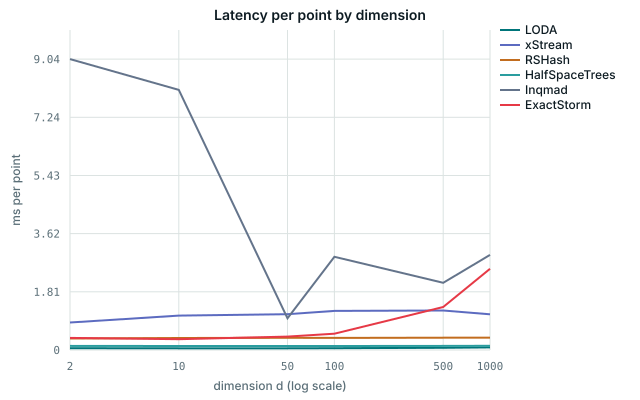
\includegraphics[width=0.8\textwidth]{dimensions.svg}
\caption{Latency per point vs. dimension (log scale). LODA and HalfSpaceTrees scale near-constantly; RSHash, xStream, Inqmad, ExactStorm show logarithmic or linear growth.}
\label{fig:dimensions}
\end{figure}

LODA and HalfSpaceTrees maintain sub-millisecond latency even at 1,000 features. RSHash's hashing cost grows with dimension. ExactStorm's distance computations scale quadratically.

\subsection{Memory Stability}
\label{sec:results_memory}

All 50+ detectors pass the 1M-point memory stability test (traced memory growth $<$ 512 KiB between checkpoints 200K and 1M). This confirms bounded memory as required for streaming deployment.

\subsection{Calibration and Alerts}
\label{sec:results_calibration}

ConformalProbabilityCalibrator achieves near-target false alert rates across thresholds. At threshold $1-\text{anomaly rate}$, the mean false alert rate matches the anomaly fraction. SPOTProbabilityCalibrator provides theoretically grounded extreme-value thresholds but requires sufficient peaks for stable fitting.

\section{Library Comparisons}
\label{sec:comparisons}

\subsection{Same-Algorithm Comparisons}
\label{sec:same_algo}

Table~\ref{tab:comparison_summary} compares PySAD implementations with equivalent algorithms in other libraries on the 17 ODDS datasets.

\begin{table}[htbp]
\centering
\caption{Same-algorithm comparison: PySAD vs. other libraries (AUROC / ms per point).}
\label{tab:comparison_summary}
\begin{tabular}{llll}
\toprule
Algorithm & PySAD & River & CapyMOA \\
\midrule
LODA & \textbf{0.790 / 0.04} & 0.754 / 0.29 & 0.715 / 1.25 \\
HalfSpaceTrees & \textbf{0.796 / 0.08} & 0.702 / 0.03 & 0.500 / 0.01 \\
IncrementalLOF & \textbf{0.675 / 0.21} & 0.675 / 14.33 & -- \\
RobustRandomCutForest & \textbf{0.787 / 8.96} & -- & 0.787 / 101.37 \\
RSHash & \textbf{0.817 / 0.27} & -- & 0.621 / 5.64 \\
OnlineOneClassSVM & \textbf{0.702 / 0.04} & 0.469 / 0.01 & -- \\
\bottomrule
\end{tabular}
\end{table}

PySAD's implementations consistently match or exceed the accuracy of other libraries while being significantly faster (7$\times$--31$\times$ for LODA, 68$\times$ for IncrementalLOF, 11$\times$ for RRCF, 21$\times$ for RSHash). The speed advantage comes from pure NumPy/SciPy implementations without JVM or Python overhead.

\subsection{Full Library Rankings}
\label{sec:full_rankings}

Figures in \texttt{docs/comparisons/} show full rankings combining PySAD detectors with each library's detectors. PySAD detectors occupy the top positions in the accuracy-speed Pareto frontier.

\section{Discussion}
\label{sec:discussion}

\subsection{Strengths of StreamBench}
\label{sec:strengths}

\begin{itemize}
    \item \textbf{Unified protocol:} All detectors, all libraries, same prequential evaluation.
    \item \textbf{Broad coverage:} Multivariate, univariate, drift, synthetic scaling, memory.
    \item \textbf{Reproducibility:} Fixed seeds, score rounding, commit tracking, CI integration.
    \item \textbf{Extensibility:} New detectors auto-discovered from \texttt{pysad.models.\_\_all\_\_}.
    \item \textbf{Open source:} BSD-3-Clause, no JVM, pure Python/NumPy/SciPy/scikit-learn.
\end{itemize}

\subsection{Limitations}
\label{sec:limitations}

\begin{itemize}
    \item \textbf{Default parameters only:} No hyperparameter tuning. Tuned parameters can change rankings significantly (e.g., KitNet's default training window exceeds 7 ODDS datasets).
    \item \textbf{Single seed:} Results can vary with seed on small datasets. Mean over seeds is more stable but increases compute.
    \item \textbf{ODDS shuffle:} Shuffling destroys temporal structure. The drift part compensates but covers only 8 streams.
    \item   \textbf{NAB calibration dependency:} Non-unit-score detectors are calibrated via ConformalProbabilityCalibrator for NAB scoring, which affects their NAB scores.
    \item \textbf{UCR subset:} Only 84/250 series (those $\le$ 20K points) are evaluated.
\end{itemize}

\subsection{Guidance for Practitioners}
\label{sec:guidance}

\begin{itemize}
    \item \textbf{First try (multivariate):} LODA (fast, parameter-light, explainable) or HalfSpaceTrees (known feature ranges).
    \item \textbf{High-dimensional:} xStream (stream hashing projection).
    \item \textbf{Drift:} DriftAdaptiveDetector wrapping any base detector.
    \item \textbf{Univariate with seasonality:} SeasonalHybridESD.
    \item \textbf{Univariate without seasonality:} MedianAbsoluteDeviation.
    \item \textbf{Subsequence discords:} DAMP or SAND.
    \item \textbf{Network/logs:} KitNet or DrainLogParser + LODA.
    \item \textbf{Existing PyOD model:} ReferenceWindowModel.
\end{itemize}

These are starting points based on method design, not benchmark rankings. Compare 2--3 candidates on your data.

\section{Conclusion}
\label{sec:conclusion}

StreamBench provides the most comprehensive benchmark for streaming anomaly detection to date, evaluating 50+ detectors across multivariate and univariate streams, with concept drift, dimensionality scaling, memory stability, and cross-library comparisons. The benchmark is fully automated, reproducible, and integrated into PySAD's development workflow.

Key findings:
\begin{itemize}
    \item PySAD's pure-NumPy implementations achieve superior accuracy-speed trade-offs compared to River, CapyMOA, and StreamAD.
    \item LocalOutlierProbability and RSHash lead in accuracy; LODA and HalfSpaceTrees lead in speed-accuracy balance.
    \item HTM and KNNCAD reproduce NAB scoreboard results; RelativeEntropy exceeds them due to paper-faithful quantization.
    \item All detectors maintain bounded memory over 1M-point streams.
    \item Dimensionality scaling favors projection-based (LODA, HalfSpaceTrees) and hashing-based (RSHash) methods.
\end{itemize}

StreamBench is open source and welcomes contributions of new detectors, datasets, and evaluation protocols.

\section*{Availability}

StreamBench is part of PySAD:
\begin{itemize}
    \item Code: \url{https://github.com/selimfirat/pysad/tree/master/benchmarks}
    \item Documentation: \url{https://pysad.readthedocs.io/en/stable/benchmark.html}
    \item Results: \url{https://github.com/selimfirat/pysad/tree/master/docs/benchmark}
    \item License: BSD-3-Clause
\end{itemize}

\section*{Acknowledgments}

We thank the authors of all cited detectors for making their algorithms available. We thank the maintainers of River, CapyMOA, StreamAD, PyOD, and Alibi Detect for their libraries. This work was supported by the PySAD open-source community.

\bibliographystyle{plainnat}
\bibliography{../docs/refs}

\end{document}